\chapter{Implementación del trabajo}
\label{chapter:implementacion}

Durante el desarrollo de este trabajo, se ha seguido un ciclo de trabajo iterativo, en el que se han ido realizando pruebas y modificaciones sobre el código, hasta obtener los resultados deseados. En este capítulo se describirán los pasos seguidos para la implementación del trabajo, así como las herramientas utilizadas para ello. Este proceso se puede dividir en las siguientes etapas:
\begin{itemize}
    \item \textbf{Preprocesamiento de datos:} en esta etapa se ha realizado manipulación y limpieza de datos, de tal forma que estos se encuentren en un formato adecuado para ser procesados por los modelos. A la par, se ha realizado un análisis exploratorio de los datos, con el fin de obtener información relevante sobre los mismos.
    \item \textbf{Aplicación de un modelo basado en YOLOv5}: en esta etapa se ha entrenado modelo basado en YOLOv5, con el fin de realizar la detección de insectos en las imágenes.
    \item \textbf{Aplicación de un modelo basado en EfficientNet}: en esta etapa se hace lo análogo a la etapa anterior, pero con un modelo basado en EfficientNet.
    \item \textbf{Evaluación de los modelos:} en esta etapa se evalúan los modelos, con el fin de determinar cuál de ellos es el más adecuado para el problema.
    \item \textbf{Reconstrucción de red de polinizadores:} en esta etapa, utilizando el modelo seleccionado, se reconstruye la red de polinizadores.
\end{itemize}

\section{Entorno de trabajo}

En general, se utilizó el lenguaje de programación Python para el desarrollo de este trabajo. En específico, se desarrolló el código en el entorno Jupyter Notebook. Para el modelo basado en YOLOv5, se utilizó la librería \textit{Pytorch}, mientras que para el modelo basado en EfficientNet, se utilizó la librería \textit{Tensorflow}. Finalmente, para la reconstrucción, análisis y visualización de la red de polinizadores, se utilizó la librería \textit{NetworkX}.

En cuanto al hardware utilizado, se emplearon dos instancias. Para el procesamiento de datos y el entrenamiento del modelo basado en EfficientNet, se utilizó un computador de escritorio con procesador AMD Rayzen 7 de 8 núcleos y 40 GB de memoria RAM, adicionalmente, se utilizó una tarjeta gráfica NVIDIA GeForce RTX 3060 de 12 GB de memoria dedicada. Sin embargo, esto no fue suficiente para los modelos basados en YOLOv5, por lo cual se utilizó Google Colab, con una GPU Nvidia A100 de 40 GB de memoria dedicada.


\section{Procesamiento de datos}


Los datos para este estudio se obtuvieron mediante un sistema de monitoreo automático desarrollado en \cite{serra-2022}, que consistió en un ensamblaje de cámara controlado por un ordenador de placa única, específicamente una Raspberry Pi 4. Esta configuración fue elegida por su óptima resolución óptica para objetos pequeños como insectos y flores, y su capacidad para programar ciclos de vídeo en el campo. El sistema incluía una cámara Module V2 de 5MP, que proporcionaba videos de 1080p a 30 fotogramas por segundo. Para la autonomía, se utilizó una batería portátil de 1000mAh Li-polímero, que permitía hasta seis horas de funcionamiento, y los videos se almacenaban en un USB de 32 GB. Todo el conjunto estaba protegido por una caja de plástico y montado en un trípode, diseñado para registrar interacciones planta-polinizador.

Para la recopilación de datos, se programó la Raspberry Pi 4 para automatizar la grabación de videos en ciclos de 10 minutos durante periodos de una hora y media, usando un archivo '.ssh' y Python 3.0. Además de los videos capturados por este sistema, se desarrolló una biblioteca fotográfica de 12000 imágenes de insectos polinizadores. Los objetos en los fotogramas de los videos se etiquetaron manualmente utilizando el programa LabelImg.

De manera específica, para este proyecto, se seleccionó 5445 imágenes de flores con polinizadores, las cuales fueron seleccionadas por el autor de \cite{serra-2022} como las de mejor calidad. Estas imágenes contaban con diferentes dimensiones, siendo mayoritario el tamaño de 1280$\times$962 píxeles. El ancho de las imágenes era fijo, y la distribución del alto de las imágenes, en escala logarítmica, se puede apreciar en la Figura~\ref{fig:dimensiones}.

\begin{figure}[H]
    \centering
    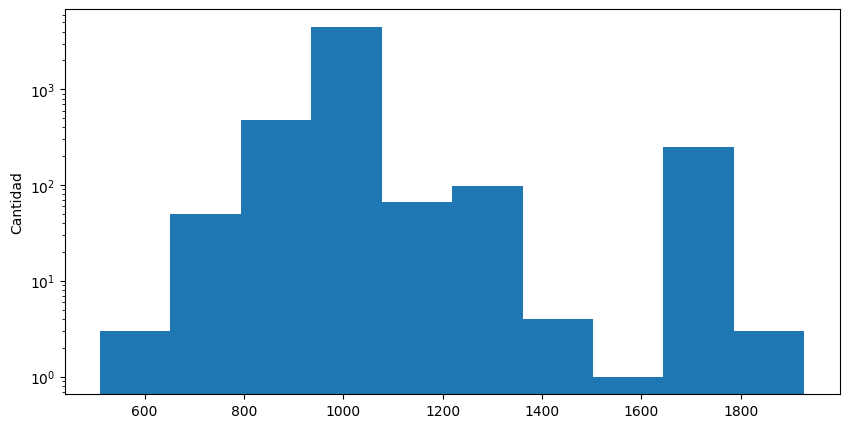
\includegraphics[width=0.8\textwidth]{Figuras/dimensiones.png}
    \caption{Distribución del alto de las imágenes, en escala logarítmica.}
    \label{fig:dimensiones}
\end{figure}

Dado que los modelos a utilizarse trabajan con imágenes del mismo tamaño, se debe estandarizar los altos de las imágenes. Para esto, se tomó como medida estándar la moda de las alturas. En las imágenes con un alto menor a este valor, se completó con un fondo blanco, mientras que en las que poseían un alto mayor a esto, se las recortó.

De cada imagen se contaba con un archivo XML, que contenía la información de las coordenadas de los polinizadores en la imagen, así como la especie de cada uno de ellos. Un ejemplo de este archivo se puede apreciar en el Código~\ref{code:xml}.

\begin{lstlisting}[language=XML, caption={Ejemplo de archivo XML de información de imágenes.}, label={code:xml}]
    <annotation>
	<folder>fotos transformades</folder>
	<filename>P1050344.JPG</filename>
	<path>F:\polinitzadors\fotos insectes\fotos transformades\P1050344.JPG</path>
	<source>
		<database>Unknown</database>
	</source>
	<size>
		<width>1280</width>
		<height>960</height>
		<depth>3</depth>
	</size>
	<segmented>0</segmented>
	<object>
		<name>Bee</name>
		<pose>Unspecified</pose>
		<truncated>0</truncated>
		<difficult>0</difficult>
		<bndbox>
			<xmin>344</xmin>
			<ymin>243</ymin>
			<xmax>569</xmax>
			<ymax>429</ymax>
		</bndbox>
	</object>
</annotation>
\end{lstlisting}

De la información de las imágenes se tomó el nombre de la imagen (\texttt{filename}), el nombre del objeto (\texttt{object, name}) y la posición (\texttt{object, bndbox}). A partir del nombre del objeto, se realizó una clasificación de los polinizadores en 7 categorías: Bee, Lepidoptera, Diptera, Coleoptera, Others, Wasp y Hoverfly. Cabe señalar que, en algunas imágenes, se encontraban más de un polinizador. En la Figura~\ref{fig:especies} se puede apreciar un ejemplo de cada una de estas categorías.

\begin{figure}[H]
    \centering
    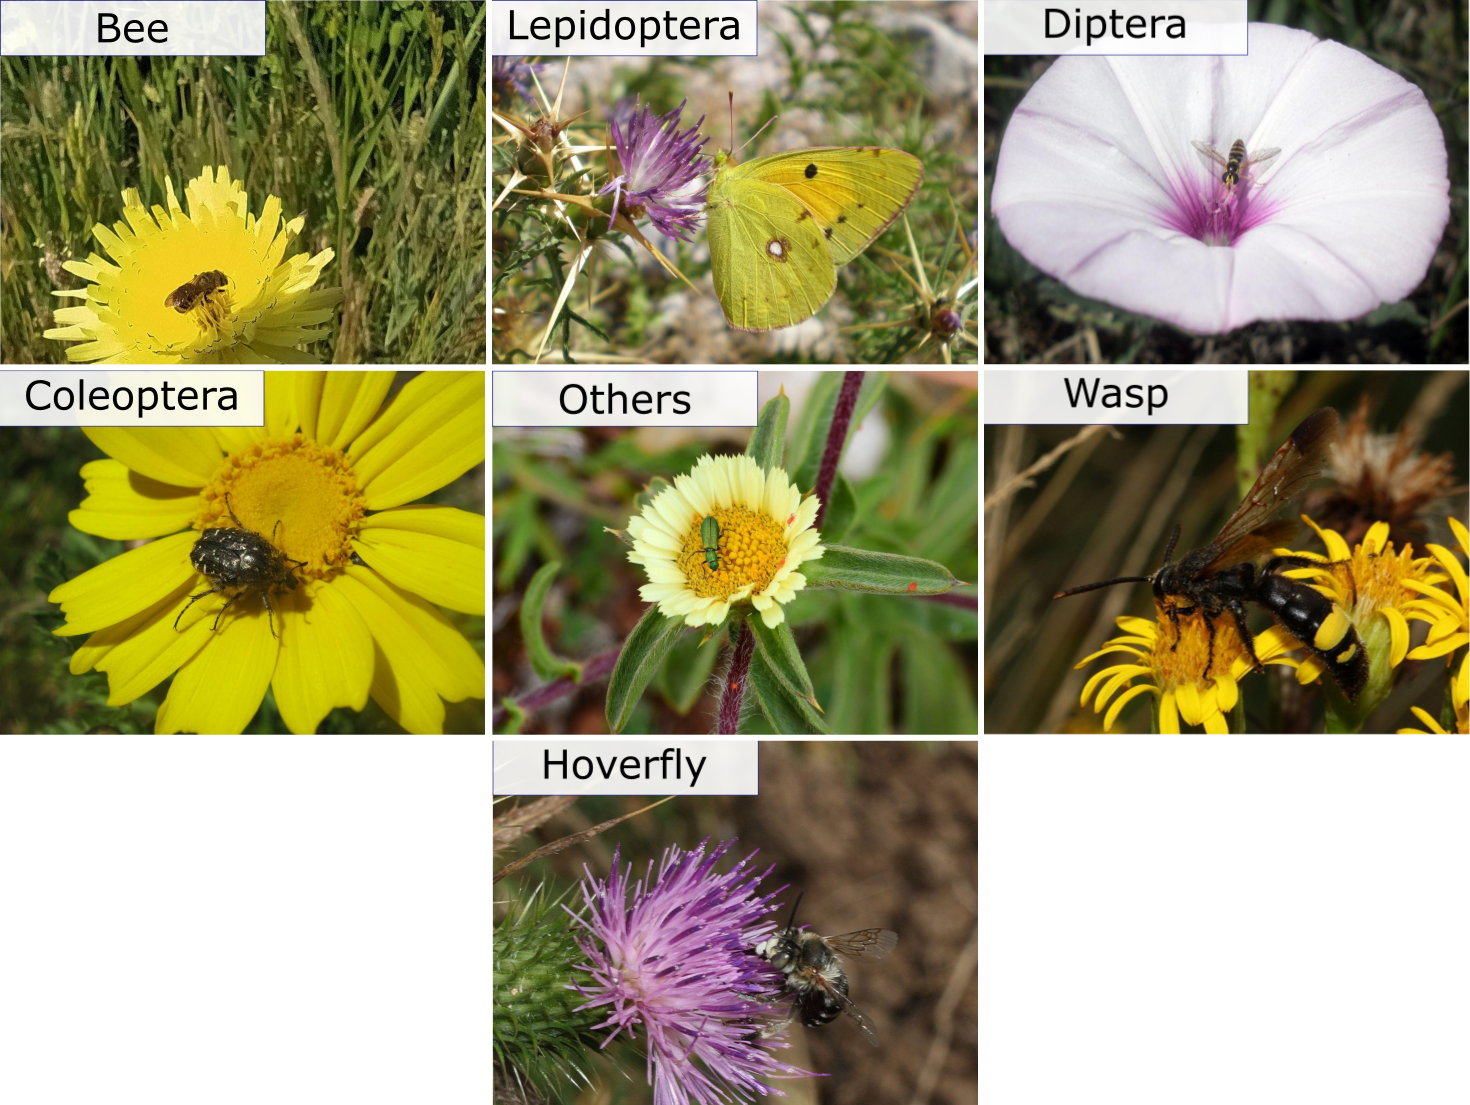
\includegraphics[width=0.95\textwidth]{Figuras/ejemplos.png}
    \caption{Ejemplo de cada una de las especies de polinizadores.}
    \label{fig:especies}
\end{figure}

La distribución de las especies, por categoría, en las imágenes se puede apreciar en la Figura~\ref{fig:distribucion_especies}, en escala logarítmica. Se observa que la especie más abundante es «Bee», con 5189, seguida de «Lepidoptera», con 510, y «Diptera», con 305. Por otro lado, las especies menos abundantes son «Wasp», con 109, y «Hoverfly», con 81. En total, en las 5445 imágenes se tienen 6681 polinizadores, por lo cual, para el modelo, se tiene en la práctica 6681 imágenes etiquetadas.

\begin{figure}[H]
    \centering
    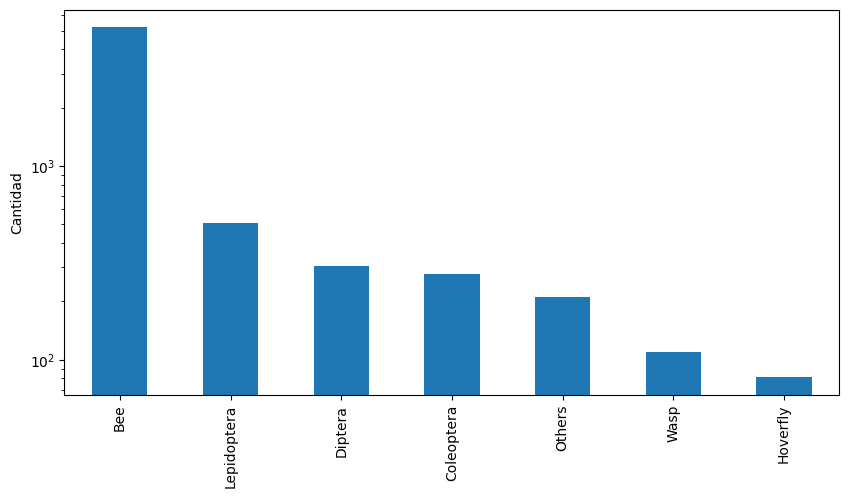
\includegraphics[width=0.79\textwidth]{Figuras/distribucion_especies.png}
    \caption{Distribución de las especies en las imágenes, en escala logarítmica.}
    \label{fig:distribucion_especies}
\end{figure}

Dada la abundante cantidad de imágenes de la especie «Bee», se decidió realizar un submuestreo de estas imágenes, con el fin de balancear la cantidad de imágenes de cada especie. Para ello, se descartaron, mediante inspección directa, imágenes similares, de una misma planta, que contenga la especie «Bee» o «Lepidoptera». El resultado de este proceso se puede apreciar en la Figura~\ref{fig:submuestreo}. De esta manera, el conjunto de datos con el que se trabajará cuenta con 2121 imágenes.

\begin{figure}[H]
    \centering
    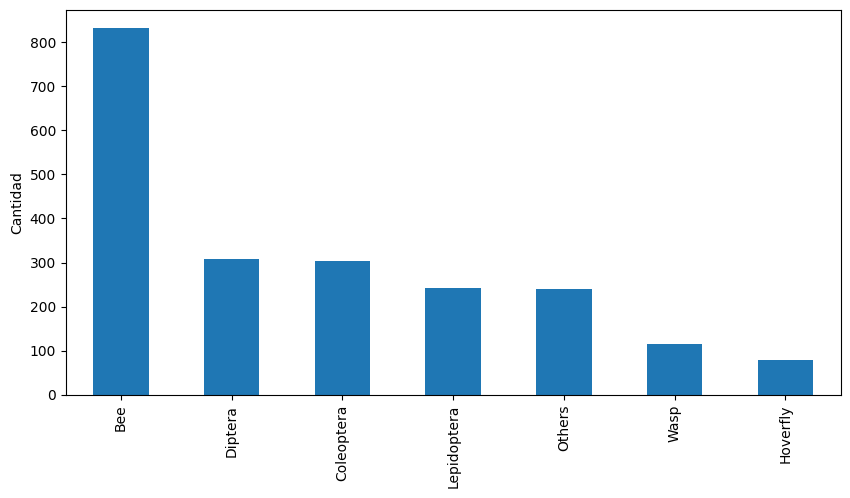
\includegraphics[width=0.79\textwidth]{Figuras/submuestreo.png}
    \caption{Submuestreo de imágenes de la categoría «Bee» y «Lepidoptera».}
    \label{fig:submuestreo}
\end{figure}


\subsection{Aumento de datos}


Para el aumento de datos, se procedió a realizar reflexiones. En las dos clases menos abundantes, «Wasp» y «Hoverfly», se realizó reflexión horizontal y vertical, mientras que en las demás clases, salvo «Bee», se realizó reflexión horizontal. En la Figura~\ref{fig:reflexiones} se puede apreciar un ejemplo de este proceso.

\begin{figure}[H]
    \centering
    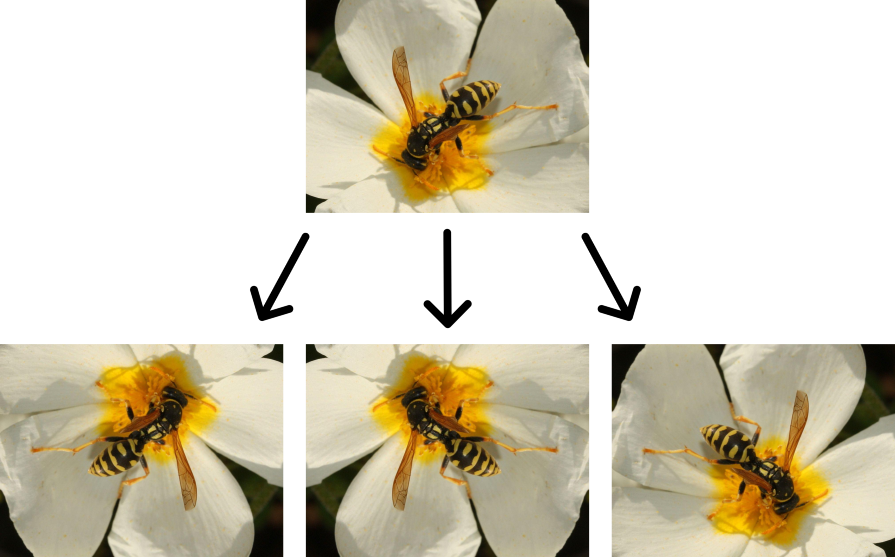
\includegraphics[width=0.75\textwidth]{Figuras/reflexion.png}
    \caption{Ejemplo de reflexiones realizadas.}
    \label{fig:reflexiones}
\end{figure}

Con esto, se obtuvieron 3415 imágenes y se mejoró la distribución de las mismas en las diferentes categorías. Esta distribución se puede apreciar en la Figura~\ref{fig:distribucion_especies_aumento}.

\begin{figure}[H]
    \centering
    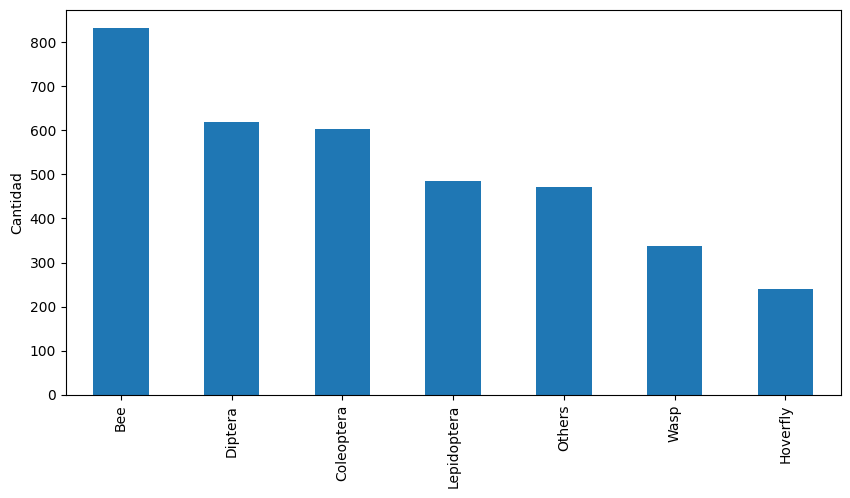
\includegraphics[width=0.8\textwidth]{Figuras/distribucion_especies_aumento.png}
    \caption{Distribución de las especies en las imágenes luego del aumento de datos.}
    \label{fig:distribucion_especies_aumento}
\end{figure}

Con estos resultados, se dividió los datos en los conjuntos de entrenamiento, validación y prueba. La distribución de los datos en estos conjuntos muestra en la Tabla~\ref{tab:distribucion_conjuntos}.

\begin{table}[H]
    \centering\small
    \begin{tabular}{cccc}
        \toprule
         & \textbf{Entrenamiento} & \textbf{Validación} & \textbf{Prueba} \\
        \midrule
        {Bee} 
        & 184 & 46 & 581 \\
        {Lepidoptera} 
        & 184 & 46 & 364 \\
        {Diptera} 
        & 184 & 46 & 322 \\
        {Coleoptera} 
        & 184 & 46 & 240 \\
        {Others} 
        & 184 & 46 & 191 \\
        {Wasp} 
        & 184 & 46 & 97 \\
        {Hoverfly} 
        & 184 & 46 & 10 \\
        \midrule
        \textbf{Total}
        & 1288 & 322 & 1805 \\
        \bottomrule
    \end{tabular}
    \caption{Distribución de los datos en los conjuntos de entrenamiento, validación y prueba.}
    \label{tab:distribucion_conjuntos}
\end{table}

\section{Aplicación de modelos}

\subsection{YOLOv5}

Para iniciar el análisis de los modelos, se procedió a realizar una prueba con el modelo YOLOv5, con el fin de determinar si este era capaz de detectar los polinizadores en las imágenes. Para ello, se utilizó el conjunto de prueba para determinar las detecciones realizadas por el modelo; cabe recalcar que, el modelo YOLOv5 está entrenado con el conjunto COCO, el cual no cuenta con polinizadores. Por esto, se obtuvieron diversos objetos detectados, los primeros diez objetos más detectados se pueden apreciar en la Tabla~\ref{tab:objetos_detectados}.

\begin{table}[H]
    \centering\small
    \begin{tabular}{cc}
        \toprule
        \textbf{Objeto} & \textbf{Cantidad} \\
        \midrule
        no detection &  853 \\
        bird         &  322 \\
        banana       &  109 \\
        dining table &   98 \\
        apple        &   67 \\
        potted plant &   25 \\
        microwave    &   19 \\
        orange       &   19 \\
        broccoli     &   18 \\
        chair        &   16 \\
        \bottomrule
    \end{tabular}
    \caption{Objetos detectados por el modelo YOLOv5.}
    \label{tab:objetos_detectados}
\end{table}

Cabe destacar que, en las detecciones, se observan pocas referentes a plantas y ninguna referente a insectos. Adicionalmente, en los casos de detección de plantas, no se encuentran relacionados con las especies que se tienen en las imágenes.

Con este resultado base, se procedió a entrenar el modelo YOLOv5 con los datos de polinizadores. Para ello, se utilizó el conjunto de entrenamiento, y se validó con el conjunto de validación. El entrenamiento se realizó con 100 épocas, con un tamaño de lote de 32 imágenes, y con un tamaño de imagen de 1280 píxeles de ancho. 

Para evaluar el rendimiento del modelo YOLOv5 entrenado, se emplearon dos tipos de gráficos basados en el conjunto de validación: las curvas de precisión-confianza y de exhaustividad-confianza.

\begin{itemize}
    \item 
    \textbf{Curvas de Precisión-Confianza (\textit{precision-confidence}):} Estas curvas ilustran la relación entre la precisión del modelo y el nivel de confianza (o probabilidad) asignado a sus predicciones. La precisión se define como la proporción de identificaciones correctas (verdaderos positivos) entre todas las identificaciones realizadas (verdaderos positivos más falsos positivos). En este gráfico, el eje horizontal representa la confianza del modelo en sus predicciones, mientras que el eje vertical muestra la precisión correspondiente a cada nivel de confianza. Un modelo ideal tendría una curva que se mantiene alta a medida que aumenta el nivel de confianza, indicando que puede mantener una alta precisión incluso cuando está muy seguro de sus predicciones.
    \item 
    \textbf{Curvas de Exhaustividad-Confianza (\textit{recall-confidence}):} Estas curvas muestran cómo la exhaustividad (o recuperación) del modelo varía con diferentes niveles de confianza. La exhaustividad se refiere a la proporción de casos positivos reales (verdaderos positivos) que el modelo ha identificado correctamente, respecto al total de casos positivos reales (verdaderos positivos más falsos negativos). En estas curvas, el eje horizontal representa la confianza, y el eje vertical muestra la exhaustividad. Una curva ideal sería aquella que se mantenga alta en todos los niveles de confianza, lo que indica que el modelo es capaz de identificar la mayoría de los casos positivos reales incluso con un alto nivel de confianza en sus predicciones.
\end{itemize}
    
En lo que respecta a la curva de precisión-confianza (Figura~\ref{fig:P_curve}), se tiene que la precisión óptima para todas las clases se alcanza a un umbral de confianza de aproximadamente 0.948, indicando un alto grado de fiabilidad del modelo en este punto. Sin embargo, las clases individuales muestran variabilidad en la precisión; «Bee» mantienen valores altos de precisión incluso a niveles bajos de confianza, sugiriendo un reconocimiento robusto, mientras que otras clases, particularmente las agrupadas en «Others», exhiben una precisión más baja, lo que puede sugerir una mayor dificultad en su detección.

\begin{figure}[H]
    \centering
    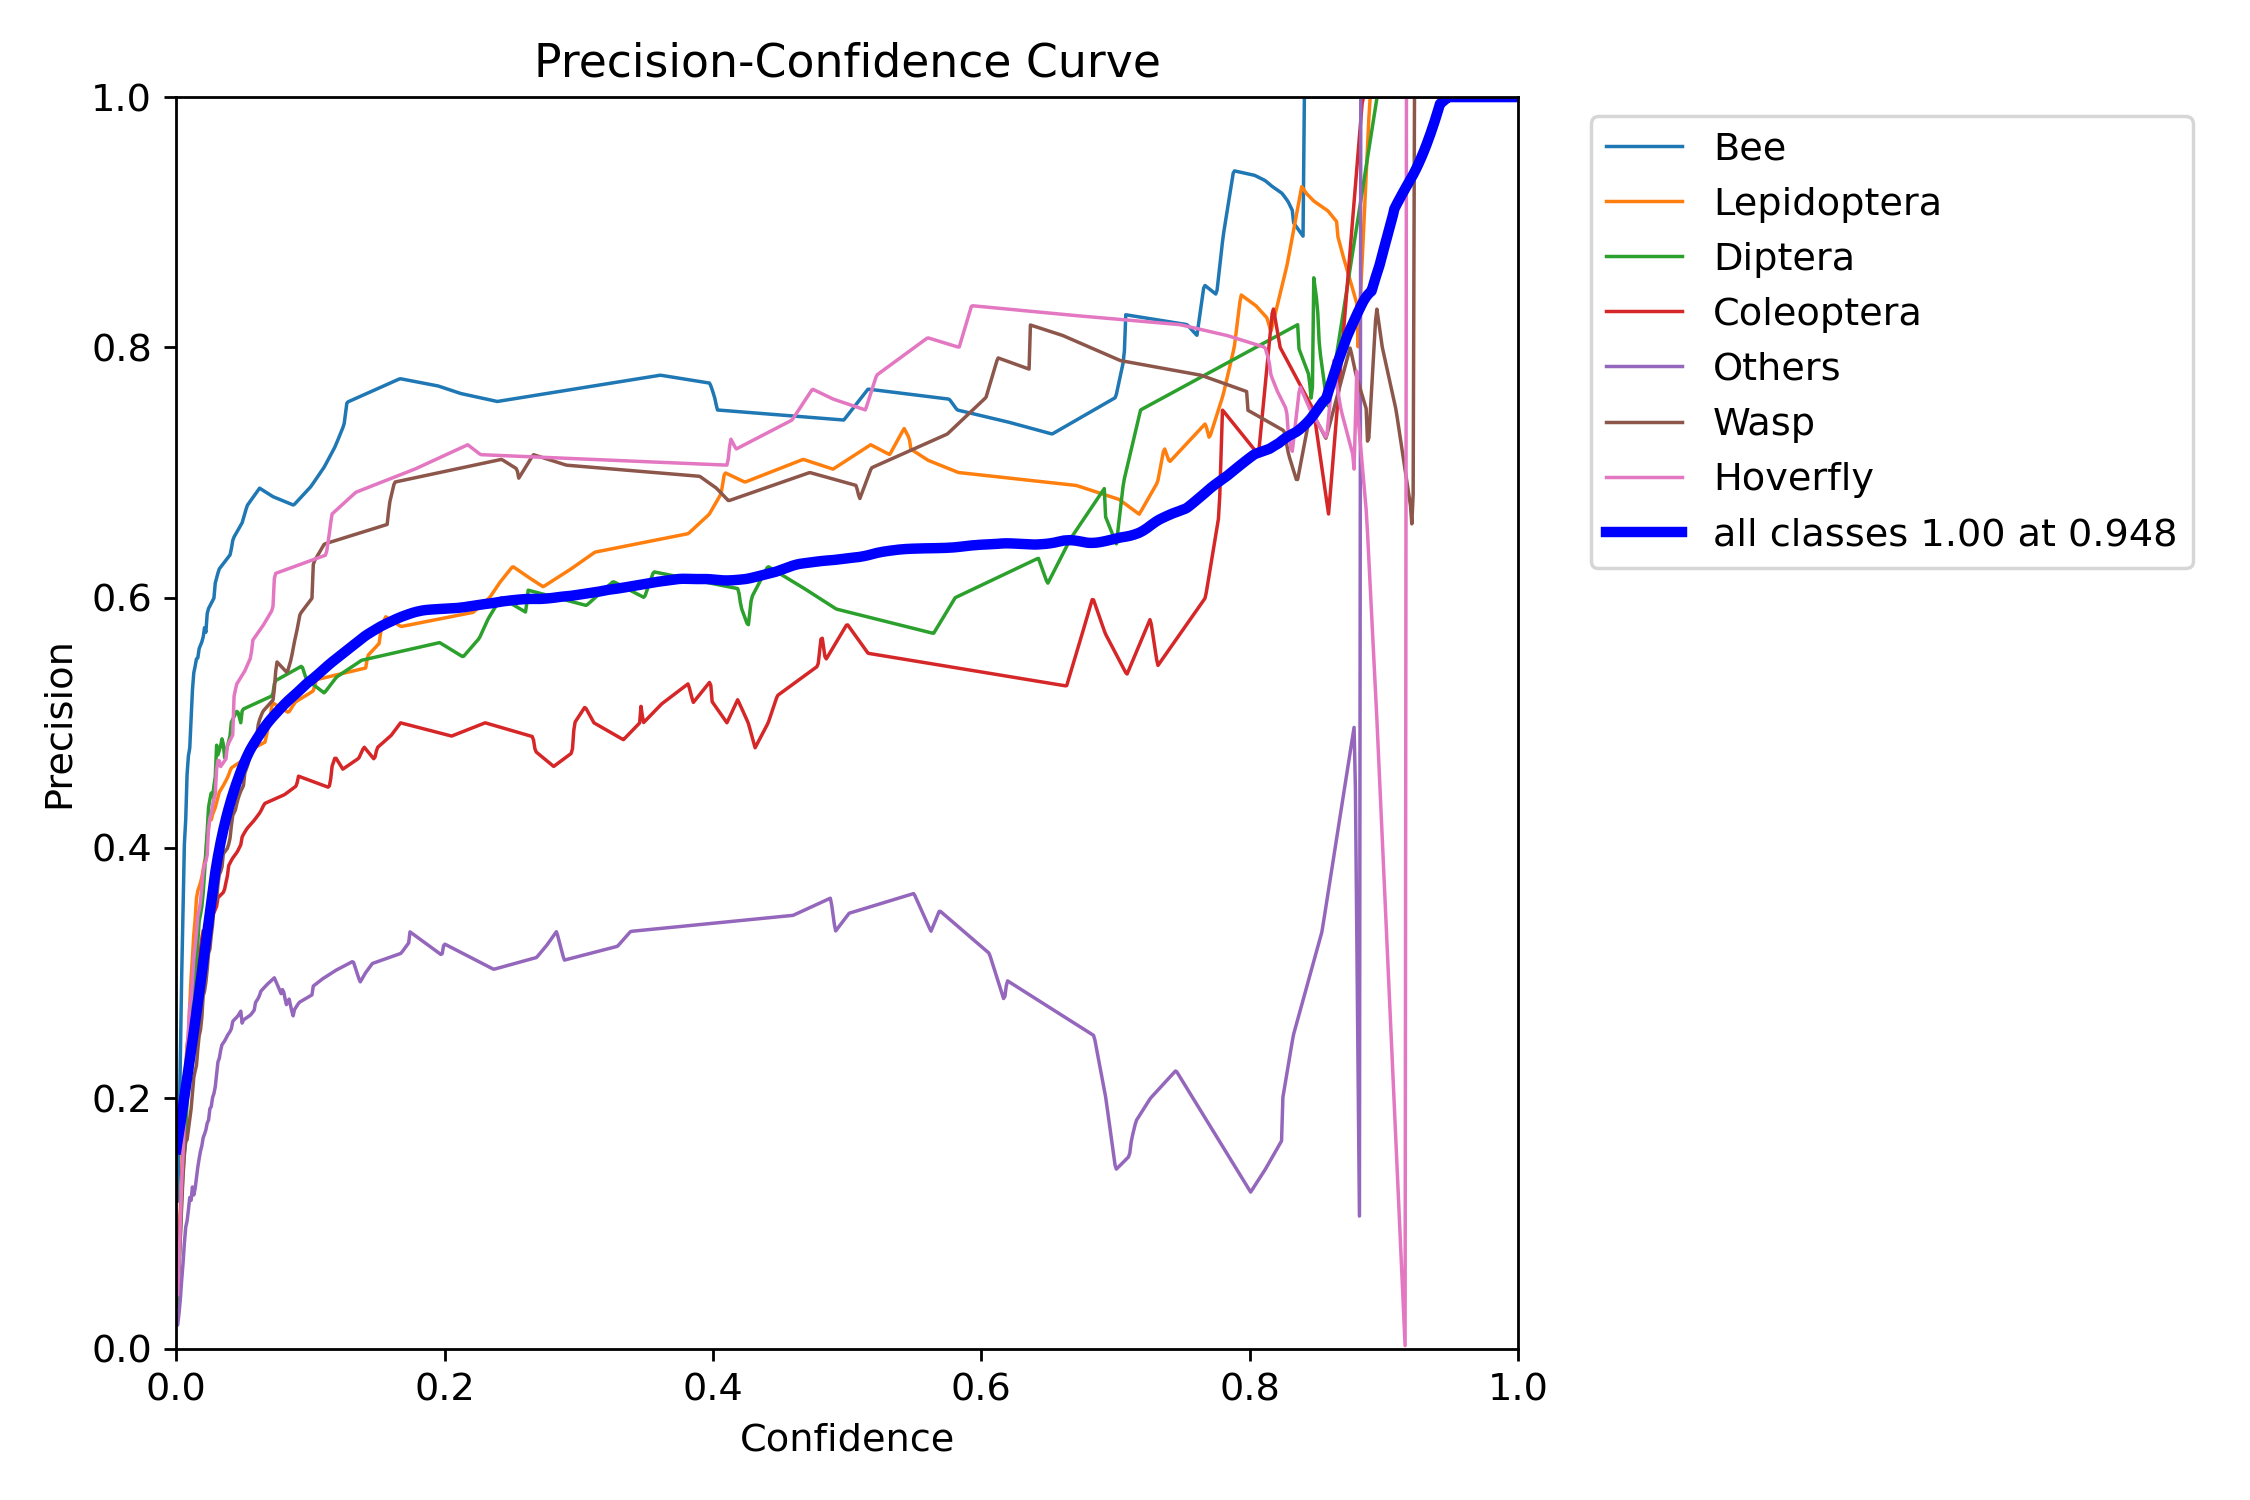
\includegraphics[width=0.85\textwidth]{Figuras/P_curve.png}
    \caption{Curvas de precisión-confianza modelo YOLOv5 en las imágenes de validación.}
    \label{fig:P_curve}
\end{figure}

\begin{figure}[H]
    \centering
    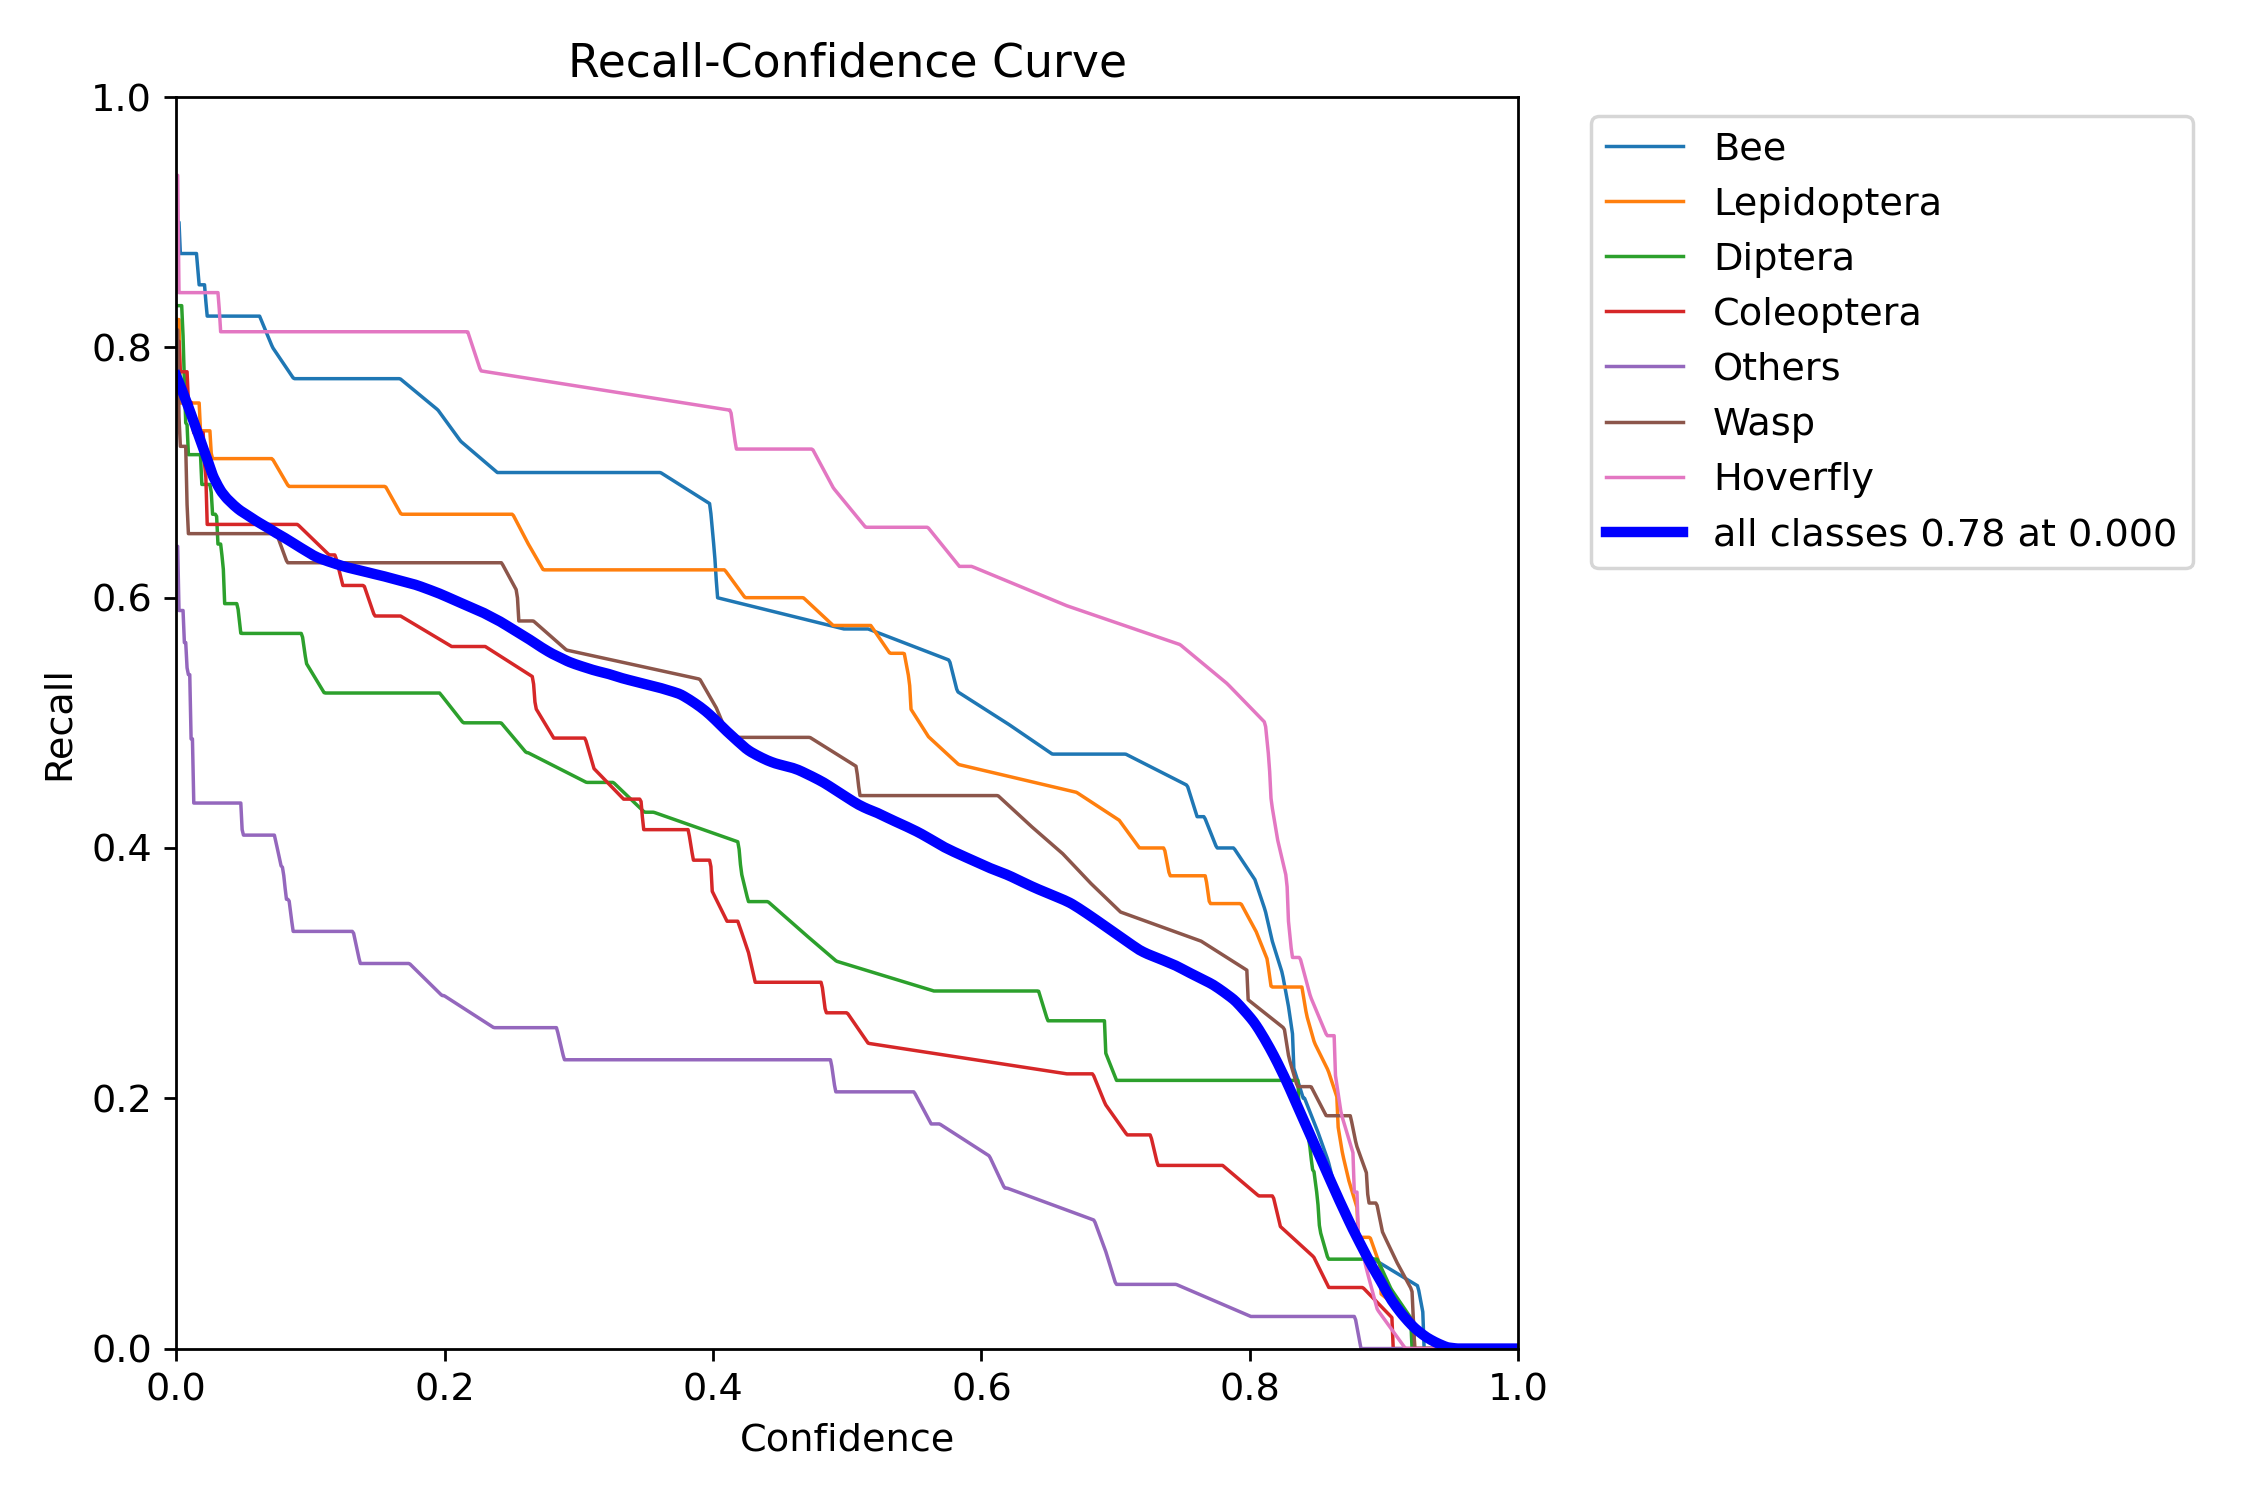
\includegraphics[width=0.85\textwidth]{Figuras/R_curve.png}
    \caption{Curvas de exhaustividad-confianza modelo YOLOv5 en las imágenes de validación.}
    \label{fig:R_curve}
\end{figure}

Por el lado de la curva exhaustividad-confianza (Figura~\ref{fig:R_curve}), demuestra que la exhaustividad general para la detección de insectos se mantiene en un nivel notable de 0.78 incluso a un umbral de confianza cero, subrayando la habilidad del modelo para detectar una gran proporción de las instancias positivas desde el inicio. Sin embargo, la exhaustividad disminuye conforme se incrementa el umbral, un comportamiento esperado al elevar la rigurosidad para la aceptación de las predicciones. Las distintas clases de insectos exhiben divergencias en la exhaustividad a lo largo de los umbrales, lo que refleja diferencias en la facilidad de detección o en la representación en el conjunto de datos.


Adicionalmente, se obtuvo la matriz de confusión con las predicciones realizadas sobre el conjunto de validación (Figura~\ref{fig:matriz_confusion_yolov5}). Se observa un alto grado de precisión en la detección de «Bee» y «Hoverlfy», con valores de 70 \% y 78 \%, respectivamente, indicando un reconocimiento efectivo de estas clases. No obstante, la confusión entre clases de insectos y el fondo, como se evidencia en los «Diptera» y «Coleoptera» mal clasificados como fondo en un 45 \% y 45 \% de los casos, respectivamente, sugiere un reto en la discriminación de características entre insectos y su entorno. Por otro lado, es remarcable el hecho de que casi no existe confusión entre las diferentes clases (valores fuera de la diagonal), llegando solo al 2 \%.

\begin{figure}[H]
    \centering
    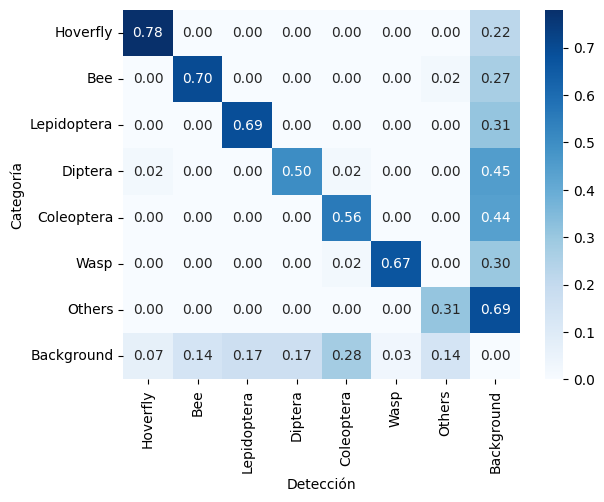
\includegraphics[width=0.75\textwidth]{Figuras/matriz_confusion_yolov5.png}
    \caption{Matriz de confusión del modelo YOLOv5.}
    \label{fig:matriz_confusion_yolov5}
\end{figure}

Por otro lado, se puede contrastar las detecciones realizadas por el modelo con las detecciones realizadas por los humanos. En la Figura~\ref{fig:comparacion_humanos_yolov5}, se puede apreciar un ejemplo de los resultados en validación. Los colores indican la clase y el valor indica la confianza de la clasificación.

\begin{figure}[H]
    \centering
    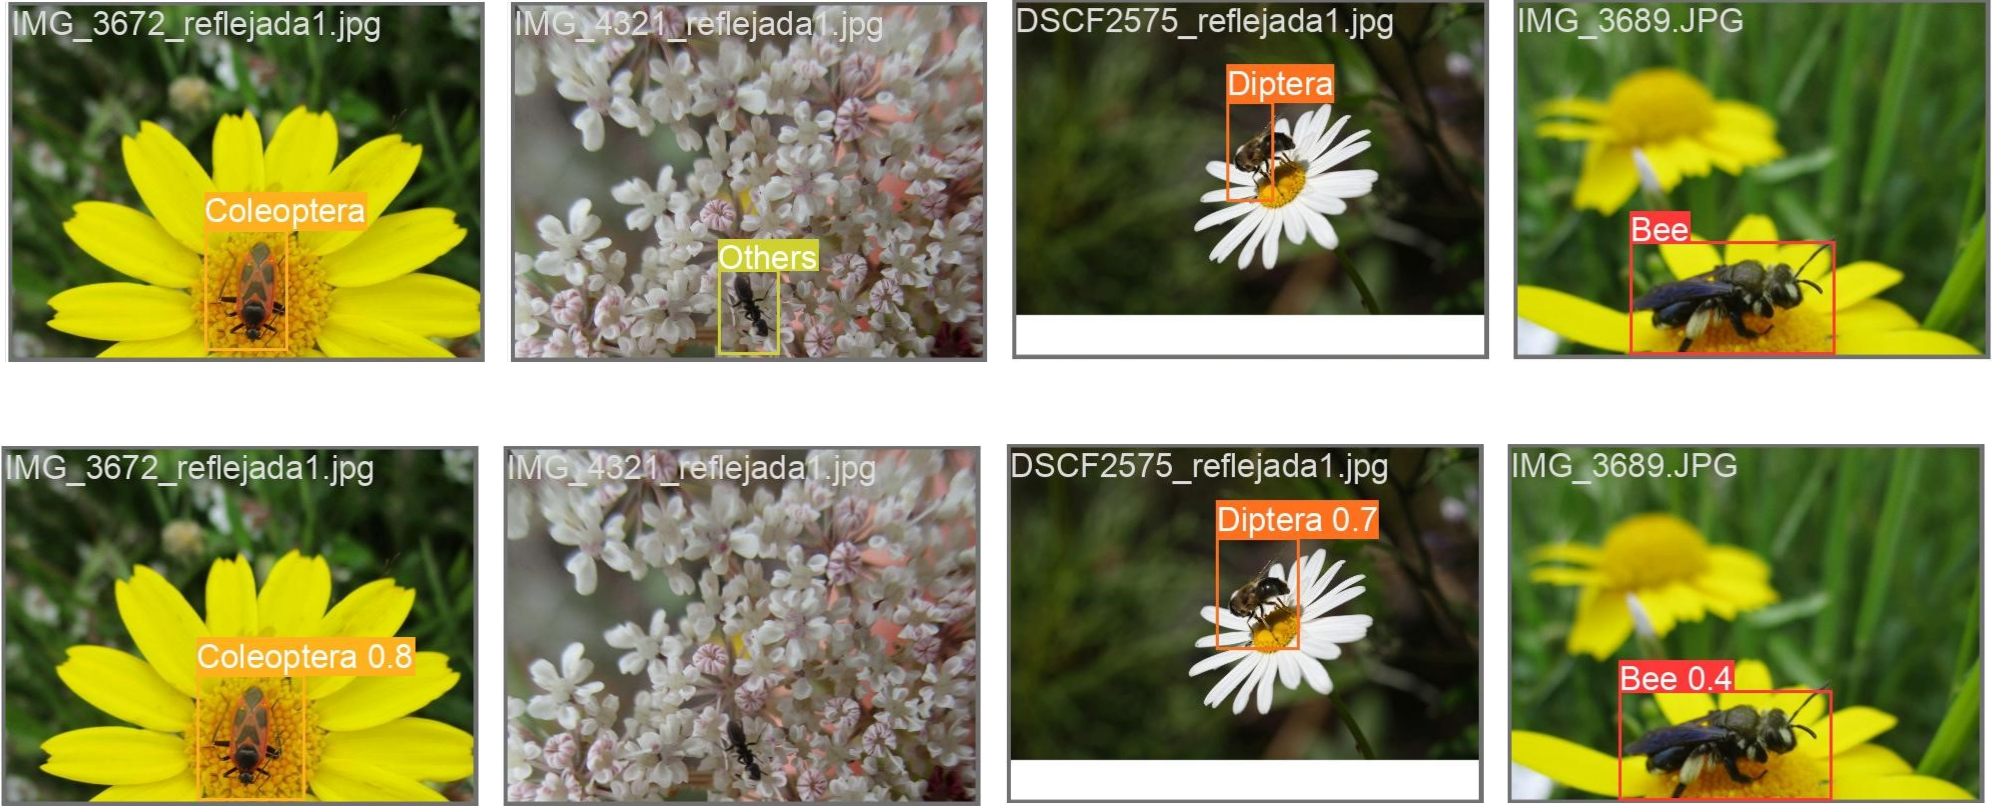
\includegraphics[width=0.98\textwidth]{Figuras/comparacion.png}
    \caption[Comparación entre detecciones realizadas por humanos y por el modelo YOLOv5.]{Comparación entre detecciones realizadas por humanos (arriba) y por el modelo YOLOv5 (abajo); el color muestra la categoría y el valor indica la confianza de la clasificación.}
    \label{fig:comparacion_humanos_yolov5}
\end{figure}


La Figura~\ref{fig:comparacion_humanos_yolov5} muestra una comparación entre la anotación manual (arriba) y las detecciones automatizadas realizadas por el modelo YOLOv5 (abajo). Es notable que en la categoría «Others», el modelo no logró detectar el insecto que sí fue identificado por un observador humano. En el caso de «Bee», el modelo proporciona un nivel de confianza relativamente bajo de 0.4, lo que podría indicar una menor certeza en su clasificación o una posible ambigüedad visual en la imagen. Sin embargo, en el caso de «Diptera», no solo la clasificación es correcta sino que la confianza es más alta (0.7), y el recuadro de detección parece más ajustado alrededor del insecto en comparación con la anotación humana. 

Finalmente, contando ya con el modelo entrenado, se procedió a realizar las detecciones en el conjunto de prueba. La matriz de confusión se puede apreciar en la Figura~\ref{fig:matriz_confusion_yolov5_prueba}. Se muestra una tendencia predominante hacia la no detección de insectos, más que hacia la confusión entre clases. Los valores significativos en la columna «Background» sugieren que el modelo frecuentemente clasifica regiones que contienen insectos como parte del fondo, particularmente en las categorías de «Coleoptera» y «Others». Sin embargo, en la confusión entre clases, se obtiene valores por debajo del 2 \%.

\begin{figure}[H]
    \centering
    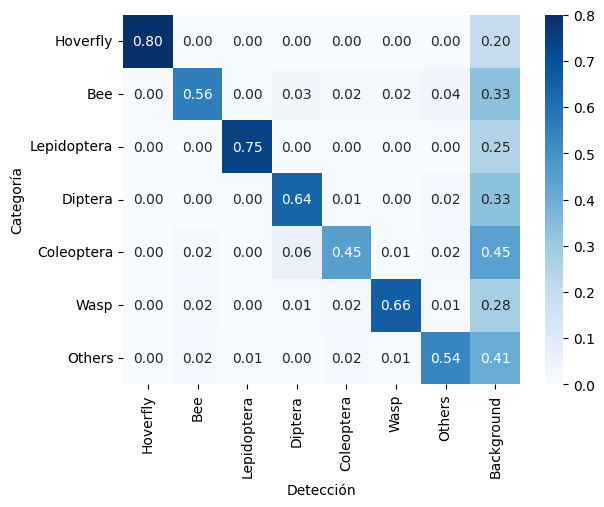
\includegraphics[width=0.75\textwidth]{Figuras/test_yolov5m_v01.png}
    \caption{Matriz de confusión del modelo YOLOv5 en el conjunto de prueba.}
    \label{fig:matriz_confusion_yolov5_prueba}
\end{figure}

Con esto, se calculó la precisión y exhaustividad por clase, los resultados pueden verse en la Tabla~\ref{tab:metricas}. La precisión se mantiene alta a través de todas las categorías, sobresaliendo en «Lepidoptera» con un 0.98, lo que refleja una fuerte capacidad del modelo para identificar correctamente las instancias positivas. No obstante, la exhaustividad presenta una variabilidad significativa; categorías como «Hoverfly» exhiben una alta concordancia entre precisión y exhaustividad (0.80), sugiriendo una detección equilibrada, mientras que otras como «Coleoptera» muestran una exhaustividad de solo 0.45, implicando una proporción considerable de falsos negativos.



\begin{table}[H]
    \centering\small
    \begin{tabular}{ccc}
        \toprule
        \textbf{Categoría} & \textbf{Precisión}  &  \textbf{Exhaustividad}\\ 
        \midrule
        Bee &  0.96 &  0.56 \\
        Coleoptera &  0.90 &  0.45 \\
        Diptera &  0.85 &  0.64 \\
        Hoverfly &  0.80 &  0.80 \\
        Lepidoptera &  0.98 &  0.75 \\
        Others &  0.79 &  0.54 \\
        Wasp &  0.82 &  0.66 \\
        \bottomrule
    \end{tabular}
    \caption{Métricas del modelo YOLOv5.}
    \label{tab:metricas}
\end{table}

\pagebreak

Adicionalmente, la exactitud global del modelo (\textit{accuracy}) es del 58 \%, lo cual refleja la proporción de predicciones correctas en relación con el total de predicciones realizadas. Este número es influido por todas las clases, por lo que la baja exhaustividad en algunas categorías puede afectar negativamente la exactitud general. 

Dado que la deficiencia del modelo se encuentra en la falta de detección de insectos en algunas imágenes, esto puede deberse a que los insectos son demasiado pequeños para ser detectados, por esta razón, se recalculó la precisión general del modelo, filtrando por el tamaño de los insectos. El cálculo de tamaño de los insectos se lo realizó tomando en cuenta el área de detección del insecto, medido en pixeles. Con esto, se obtuvieron los resultados que se presentan en la Tabla~\ref{tab:metricas_area}.

\begin{table}[H]
    \centering\small
    \begin{tabular}{ccc}
    \toprule
          \textbf{Área mínima (\%)} & \textbf{Cantidad de imágenes}  &  \textbf{Exactitud general}\\ 
    \midrule
        0.0 & 1891 & 0.58 \\
        0.1 & 1795 & 0.61 \\
        0.5 & 1489 & 0.66 \\
        1.0 & 1233 & 0.67 \\
        2.5 & 812 & 0.71 \\
        5.0 & 502 & 0.72 \\
        10.0 & 271 & 0.74 \\
    \bottomrule
    \end{tabular}
    \caption{Precisión general modelo YOLOv5 en función del área de detección.}
    \label{tab:metricas_area}
\end{table}

Con estos resultados se observa que, el tamaño del insecto incide de manera significativa en la precisión general de la clasificación. Un posible valor para tomar es que el insecto ocupe un espacio superior al 2.5 \% del área total de la imagen, en la cual se obtiene una exactitud general de 0.71. Con esto, se recalculó la matriz de confusión, la cual se puede apreciar en la Figura~\ref{fig:matriz_confusion_yolov5_prueba_area}. Adicionalmente, se recalculó la precisión y exhaustividad por clase, los resultados pueden verse en la Tabla~\ref{tab:metricas_area}. 


La nueva matriz de confusión (Figura~\ref{fig:matriz_confusion_yolov5_prueba_area}) tras el ajuste en el tamaño de los insectos detectados refleja una mejora notable en la detección de la categoría «Hoverfly», alcanzando una precisión del 100 \%. Adicionalmente, la todas las categorías, salvo «Others», muestran una mejora en los resultados, superando en todas el valor de 0.6. Aunque la no detección ha disminuido todas las categorías, persiste como un problema significativo, especialmente en «Others».

\begin{figure}[H]
    \centering
    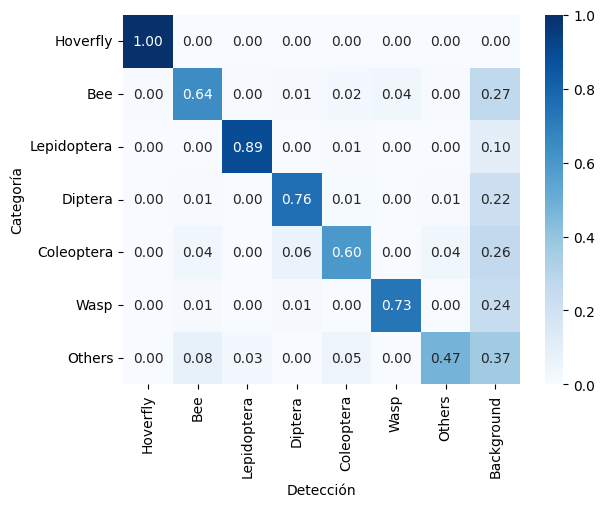
\includegraphics[width=0.75\textwidth]{Figuras/test_yolov5m_v01_area.png}
    \caption{Matriz de confusión del modelo YOLOv5 en el conjunto de prueba, con un área mínima del 2.5 \% del área total de la imagen.}
    \label{fig:matriz_confusion_yolov5_prueba_area}
\end{figure}


Por otro lado, el modelo muestra una mejora en la precisión para la mayoría de las categorías (ver Tabla~\ref{tab:metricas_area25}), con «Lepidoptera» alcanzando una precisión sobresaliente de 0.98 y una exhaustividad de 0.87.  Las categorías «Bee», «Coleoptera», y «Wasp» muestran una precisión alta, pero persiste un nivel de exhaustividad bajo, lo que indica que aún se pasan por alto instancias reales. La categoría «Others» continúa siendo la más desafiante para el modelo, con las métricas más bajas en precisión y exhaustividad, reflejando dificultades tanto en la detección como en la clasificación correcta.

\begin{table}[H]
    \centering\small
    \begin{tabular}{ccc}
    \toprule
          \textbf{Categoría} & \textbf{Precisión}  &  \textbf{Exhaustividad}\\ 
    \midrule
        Bee &  0.94 &  0.64 \\
        Coleoptera &  0.88 &  0.60 \\
        Diptera &  0.92 &  0.76 \\
        Hoverfly &  0.88 &  1.00 \\
        Lepidoptera &  0.98 &  0.87 \\
        Others &  0.72 &  0.47 \\
        Wasp &  0.86 &  0.73 \\
    \bottomrule
    \end{tabular}
    \caption{Métricas del modelo YOLOv5, con un área mínima del 2.5 \% del área total de la imagen.}
    \label{tab:metricas_area25}
\end{table}

\subsubsection{Validación cruzada}

Se implementó un enfoque de validación cruzada con 5 \textit{folds} para evaluar la generalización del modelo YOLOv5 en la tarea de clasificación. Este método consiste en dividir el conjunto de datos de forma aleatoria en cinco partes (o \textit{folds}), utilizando cuatro de ellas para el entrenamiento y la restante para la validación, repitiendo este proceso cinco veces de manera que cada \textit{folds} sirva una vez como conjunto de validación. 

Para integrar los resultados de los cinco modelos generados en la validación cruzada, se adoptó el criterio de unificarlos bajo la máxima media del nivel de confianza de las predicciones de cada modelo. Esto significa que, para cada observación, se seleccionó la predicción con la mayor confianza promedio entre los diferentes modelos. Este enfoque maximiza la certeza en las predicciones finales y contribuye a una evaluación más precisa de la estabilidad del modelo.

Con esto, se calculó la precisión y exhaustividad por clase, los resultados pueden verse en la Tabla~\ref{tab:metricas_cross}.

\begin{table}[H]
    \centering\small
    \begin{tabular}{ccc}
    \toprule
          \textbf{Categoría} & \textbf{Precisión}  &  \textbf{Exhaustividad}\\ 
    \midrule
        Bee &           0.89 &  0.69 \\
        Coleoptera &    0.91 &  0.55 \\
        Diptera &       0.85 &  0.70 \\
        Hoverfly &      0.32 &  0.70 \\
        Lepidoptera &   0.96 &  0.78 \\
        Others &        0.68 &  0.57 \\
        Wasp &          0.75 &  0.77 \\
    \bottomrule
    \end{tabular}
    \caption{Métricas del modelo YOLOv5, con validación cruzada.}
    \label{tab:metricas_cross}
\end{table}

Se presentan variaciones interesantes en comparación con los resultados originales. En la categoría «Bee», se observa una disminución en la precisión (de 0.96 a 0.89) pero un aumento en la exhaustividad (de 0.56 a 0.69), lo que indica una mejor identificación de esta categoría a costa de una precisión ligeramente reducida. Similarmente, en «Coleoptera» y «Diptera», la precisión se mantiene alta, con un notable aumento en la exhaustividad para «Diptera». Sin embargo, la categoría «Hoverfly», aunque muestra un aumento en la exhaustividad, tiene una precisión significativamente baja, posiblemente debido al número limitado de muestras. En contraste, la categoría «Others» muestra un descenso tanto en precisión como en exhaustividad.

La exactitud global del modelo mejoró notablemente, pasando de 0.58 en los resultados originales a 0.67 en la validación cruzada. Este incremento es un indicador positivo de que el modelo generaliza mejor sus predicciones a través de diferentes conjuntos de datos, lo que sugiere una robustez incrementada. Las fluctuaciones en precisión y exhaustividad, aunque son comunes en el proceso de validación y pruebas, indican que el modelo mantiene una buena capacidad de generalización. La mejora en la exactitud global, junto con los ajustes observados en otras métricas, sugiere que el modelo es confiable y efectivo, con un nivel de \textit{overfitting} controlado.

\subsection{EfficientNet}

Se siguió la misma metodología que en el modelo anterior. Se realizó una prueba con el modelo EfficientNetB7, con el fin de determinar si este era capaz de detectar los polinizadores en las imágenes. Para ello, se utilizó el conjunto de prueba para determinar las detecciones realizadas por el modelo; cabe recalcar que, el modelo EfficientNet \cite{tan-2019} está entrenado con el conjunto ImageNet, el cual no cuenta con polinizadores. Por esto, se obtuvieron diversos objetos detectados, los primeros diez objetos más detectados se pueden apreciar en la Tabla~\ref{tab:objetos_detectados_efficientnet}.

\begin{table}[H]
    \centering
    \begin{tabular}{cc}
        \toprule
        \textbf{Objeto} & \textbf{Cantidad} \\
        \midrule
        matchstick        &    779 \\
        jack-o'-lantern   &    233 \\
        nematode          &    181 \\
        daisy             &     80 \\
        abaya             &     66 \\
        spotlight         &     54 \\
        velvet            &     49 \\
        feather boa       &     31 \\
        candle            &     22 \\
        sea urchin        &     21 \\
        \bottomrule
    \end{tabular}
    \caption{Objetos detectados por el modelo EfficientNet.}
    \label{tab:objetos_detectados_efficientnet}
\end{table}

Con este resultado base, se procedió a entrenar el modelo EfficientNet con los datos de polinizadores. Para ello, se utilizó el conjunto de entrenamiento, y se validó con el conjunto de validación. El entrenamiento se realizó con 50 épocas, con un tamaño de lote de 32 imágenes, y con un tamaño de imagen de 600 píxeles, para esto, se realizó un reescalado de las imágenes. Adicionalmente, se agregó una capa \textit{softmax} al final del modelo, con el fin de realizar la clasificación de las detecciones.

Las curvas de aprendizaje obtenidas se pueden apreciar en la Figura~\ref{fig:curvas_aprendizaje_efficientnet}. Estas curvas muestran una precisión de entrenamiento y validación inusualmente bajas, lo que sugiere un posible subajuste y la necesidad de una optimización en el proceso de entrenamiento. La baja precisión, con valores fluctuantes entre 0.11 y 0.18, indica que el modelo tiene dificultades para captar las características distintivas de los datos.

\begin{figure}[H]
    \centering
    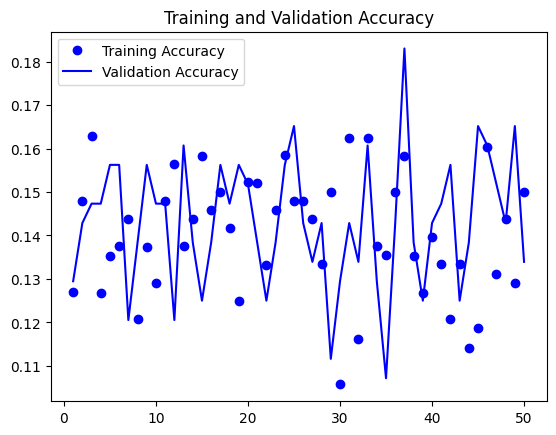
\includegraphics[width=0.49\textwidth]{Figuras/curvas_aprendizaje_efficientnet_1.png}
    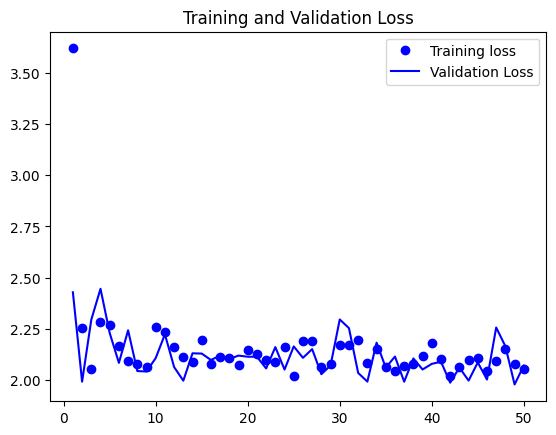
\includegraphics[width=0.49\textwidth]{Figuras/curvas_aprendizaje_efficientnet_2.png}
    \caption{Curvas de aprendizaje del modelo EfficientNet.}
    \label{fig:curvas_aprendizaje_efficientnet}
\end{figure}

Se puede apreciar que no existe un aprendizaje, esto puede deberse a que EfficientNet no toma en cuenta el bounding box de las imágenes, por lo que realiza una detección en general de la imagen, y no de los polinizadores en específico. Finalmente, contando ya con el modelo entrenado, se procedió a realizar las detecciones en el conjunto de prueba, sin resultados satisfactorios.

\section{Reconstrucción de red de polinizadores}

Con el modelo YOLOv5 entrenado, se procedió a realizar las detecciones en el conjunto de prueba. En este punto, solo se tomaron las imágenes originales, sin sus reflexiones. Se tiene un total de 1110 imágenes. Dentro de estas, el modelo detectó insectos en 701 imágenes. La distribución de los insectos en las imágenes se puede apreciar en la Figura~\ref{fig:distribucion_insectos}. Se observa que se tiene una distribución similar entre las observaciones reales y las estimaciones del modelo YOLOv5 para la mayoría de las categorías de insectos, lo que valida el buen funcionamiento del método aplicado. Sin embargo, es notable la discrepancia en la categoría «Bee», donde el modelo subestima claramente su presencia.

\begin{figure}[H]
    \centering
    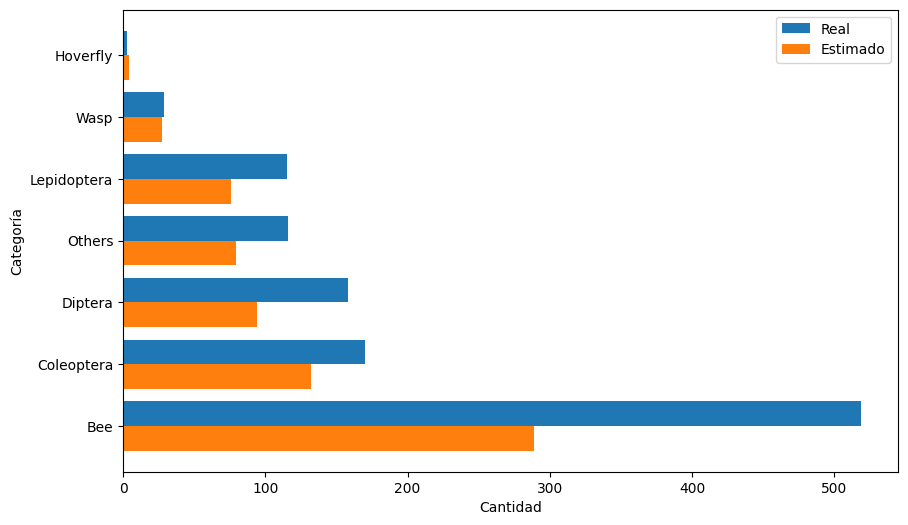
\includegraphics[width=0.835\textwidth]{Figuras/distribucion_insectos.png}
    \caption{Distribución de los insectos en las imágenes.}
    \label{fig:distribucion_insectos}
\end{figure}


Por el lado de las plantas, se utilizó la herramienta \textit{My PlantNet API} \cite{PlantNet} para la identificación de las plantas en las imágenes. A partir de los datos proporcionados por la API, se tomó la Familia de cada planta. En total, se detectaron 40 familias de plantas, la distribución de estas se puede apreciar en la Figura~\ref{fig:distribucion_familias}. Se puede apreciar que, la familia más abundante es \textit{Asteraceae}, con más de 300 imágenes. Por otro lado, existen algunas familias con una sola imagen.

\begin{figure}[H]
    \centering
    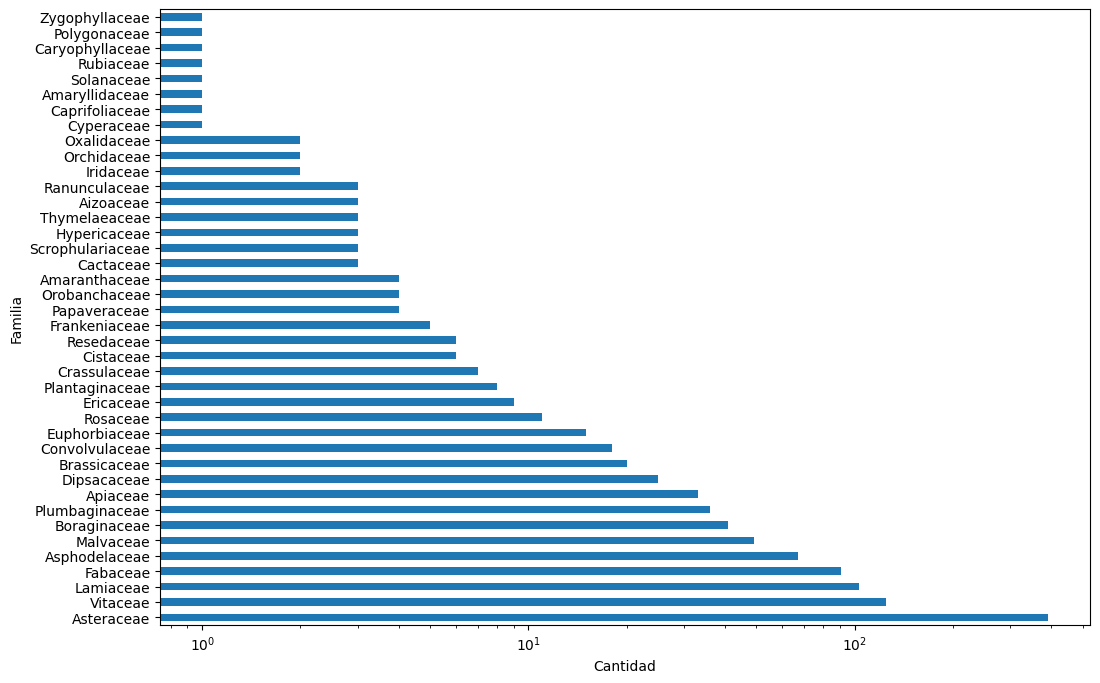
\includegraphics[width=0.885\textwidth]{Figuras/distribucion_familias.png}
    \caption{Distribución de las familias de plantas en las imágenes, en escala logarítmica.}
    \label{fig:distribucion_familias}
\end{figure}

Con esto, se llevó a cabo la construcción de dos redes planta-polinizador distintas. La primera red se derivó de las categorías identificadas a través de la observación humana, la cual se asume como el punto de referencia o red «real». Esta red proporciona una base para comparar la efectividad de las detecciones automáticas. La segunda red se generó a partir de las detecciones realizadas por el modelo YOLOv5. Al contrastar las dos redes, se puede evaluar no solo la capacidad de detección del modelo sino también su aplicabilidad en estudios ecológicos reales.

\subsection{Red planta-polinizador real}

La matriz de interacciones de la red real se puede apreciar en la Figura~\ref{fig:matriz_interacciones_real}. Se puede observar que, la mayoría de las especies interactúan con la especie «Bee», mientras que las especies «Hoverfly» y «Wasp» tienen pocas interacciones. 

\begin{figure}[H]
    \centering
    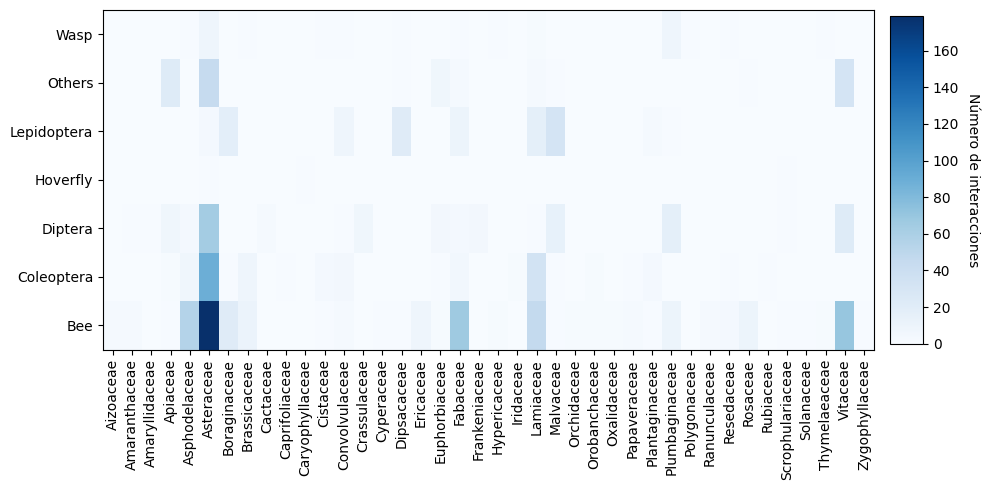
\includegraphics[width=0.96\textwidth]{Figuras/matriz_interacciones_real.png}
    \caption{Matriz de interacciones de la red real.}
    \label{fig:matriz_interacciones_real}
\end{figure}

A partir de esta matriz, con la metodología expuesta en el Capítulo~\ref{chapter:arte}, perteneciente a Young et al. \cite{young-2021}, se procedió a estimar la red real. El resultado de aplicar esta metodología es una matriz que contiene la probabilidad de conexión en el grafo, es decir, la probabilidad de que un insecto sea un polinizador de una planta. Esta matriz se puede apreciar en la Figura~\ref{fig:matriz_probabilidades_real}. 

\begin{figure}[H]
    \centering
    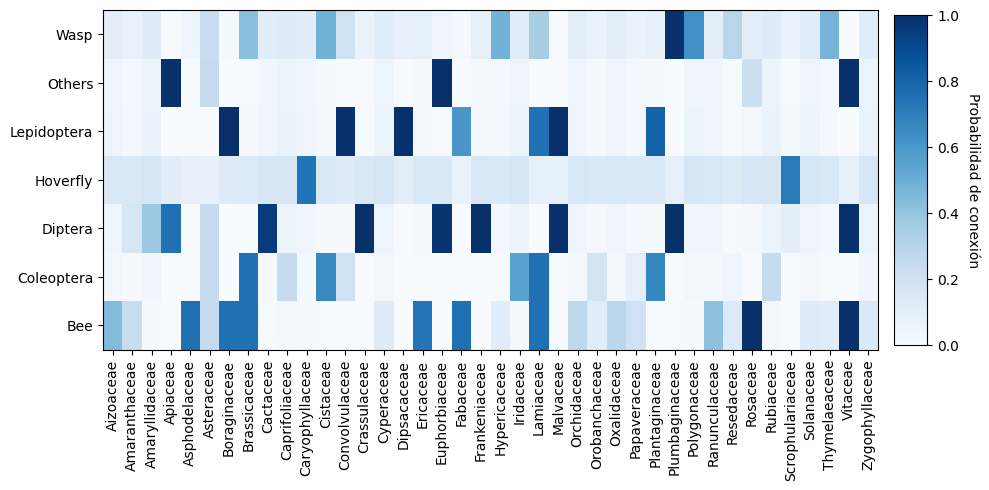
\includegraphics[width=0.96\textwidth]{Figuras/matriz_probabilidades_real.png}
    \caption{Matriz de probabilidades de la red real.}
    \label{fig:matriz_probabilidades_real}
\end{figure}

Seleccionando un umbral de confianza del 70 \%, se construyó la red planta-polinizador considerada como la red real. Este valor se eligió estratégicamente por ser el más alto que garantiza que cada especie de insecto conserva al menos una interacción con una planta, asegurando así la integridad biológica de la red. La visualización del resultado de esta estimación se presenta en la Figura~\ref{fig:red_real}. Con esto, se tiene que los insectos son polinizadores de únicamente 20 familias de plantas.

\begin{figure}[H]
    \centering
    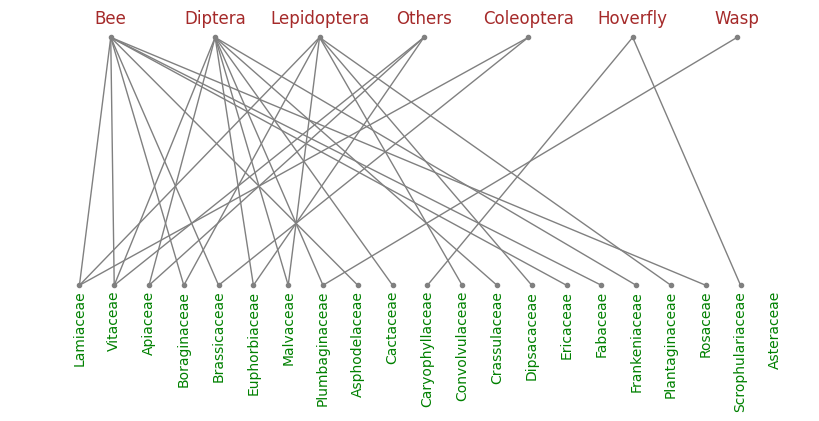
\includegraphics[width=0.95\textwidth]{Figuras/red_real.png}
    \caption{Red planta-polinizador real.}
    \label{fig:red_real}
\end{figure}


\subsection{Red planta-polinizador estimada}

La matriz de interacciones de la red estimada se puede apreciar en la Figura~\ref{fig:matriz_interacciones_estimada}. Se puede apreciar que tiene las mismas características que la matriz de interacciones de la red real, con la diferencia de que, en esta matriz, la clase «Coleoptera» posee menos interacciones que en la matriz de la red real.

\begin{figure}[H]
    \centering
    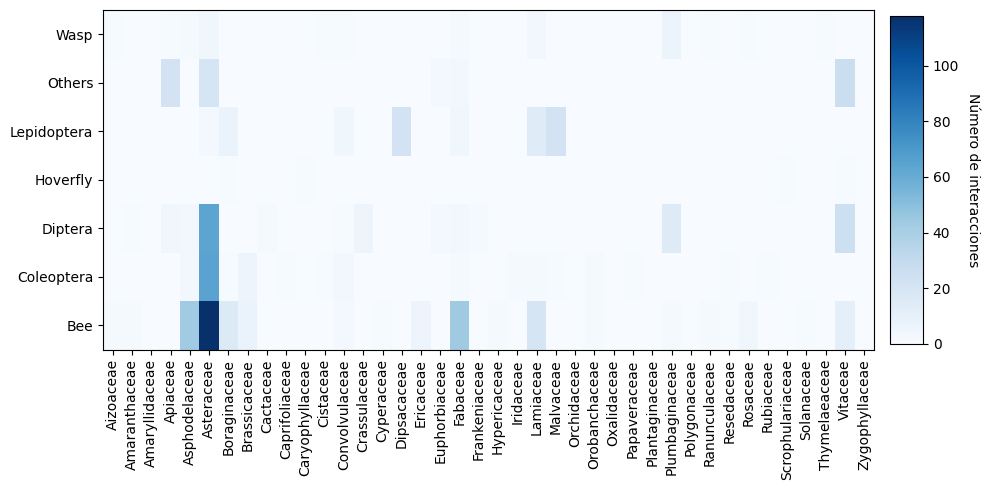
\includegraphics[width=0.96\textwidth]{Figuras/matriz_interacciones_estimada.png}
    \caption{Matriz de interacciones de la red estimada.}
    \label{fig:matriz_interacciones_estimada}
\end{figure}

A partir de esta matriz, al igual de lo descrito en la sección anterior, se procedió a estimar la red estimada. Con esto, se obtuvo la matriz de probabilidades de la red estimada, la cual se puede apreciar en la Figura~\ref{fig:matriz_probabilidades_estimada}.

\begin{figure}[H]
    \centering
    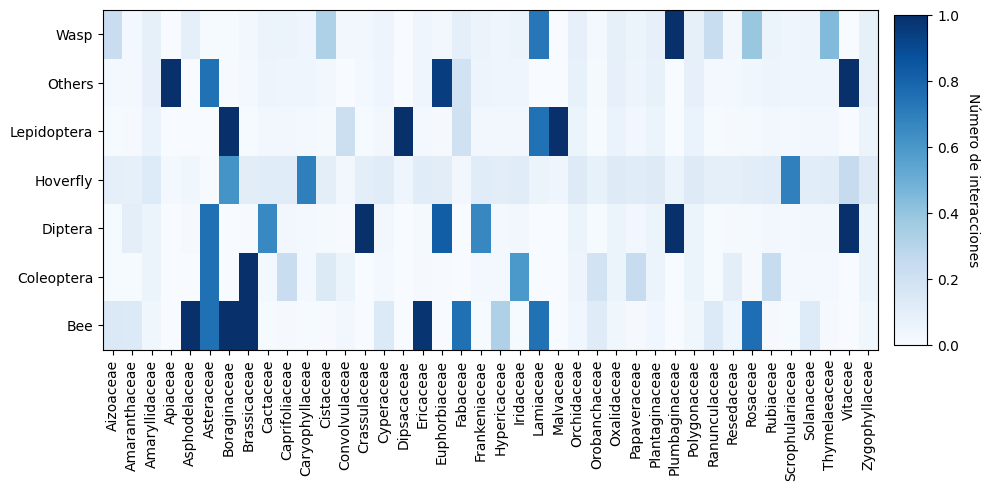
\includegraphics[width=0.96\textwidth]{Figuras/matriz_probabilidades_estimada.png}
    \caption{Matriz de probabilidades de la red estimada.}
    \label{fig:matriz_probabilidades_estimada}
\end{figure}

Tomando un nivel de confianza del 70 \%, se procedió a generar la red estimada. El resultado de esta estimación se puede apreciar en la Figura~\ref{fig:red_estimada}.

\begin{figure}[H]
    \centering
    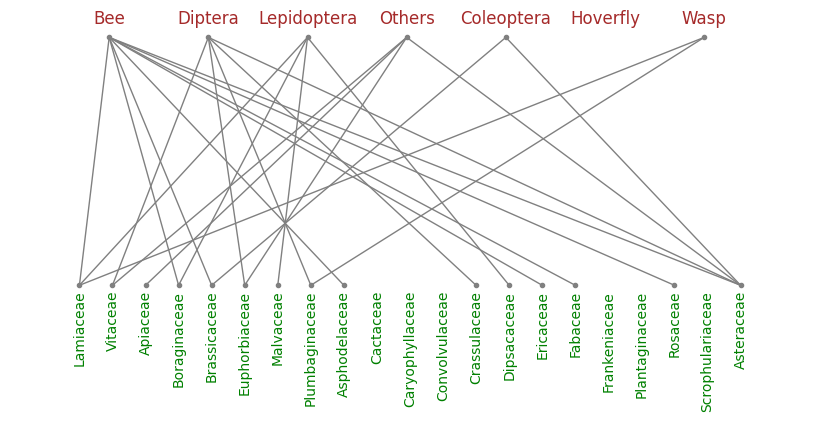
\includegraphics[width=0.95\textwidth]{Figuras/red_estimada.png}
    \caption{Red estimada.}
    \label{fig:red_estimada}
\end{figure}



\section{Comparación de redes}

Para la comparación de las redes, se tomará la componente conexa máximas de cada red. Para una comparación visual, se presentan la gráfica de ambas redes en la Figura~\ref{fig:redes_comparacion}. 

\begin{figure}[H]
    \centering
    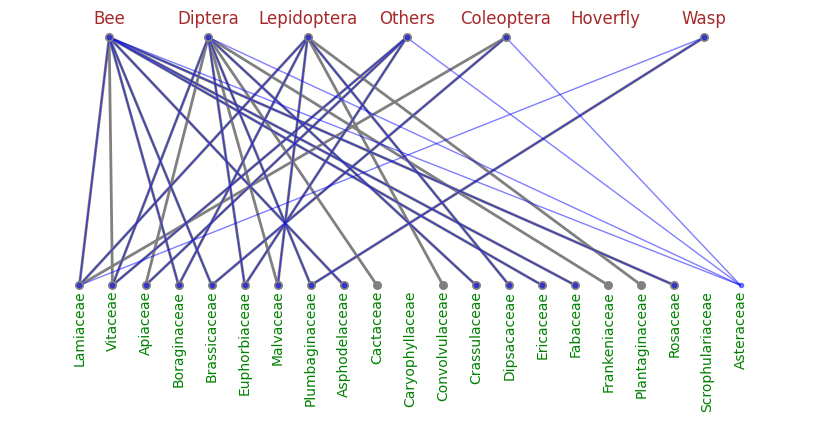
\includegraphics[width=0.95\textwidth]{Figuras/redes_comparacion.png}
    \caption[Comparación de las redes real y estimada.]{Comparación de las redes, en gris la red real y en azul la red estimada.}
    \label{fig:redes_comparacion}
\end{figure}

Se puede apreciar que, la red estimada posee una mayor cantidad de nodos y aristas que la red real. Por otro lado, se observa que, en la red estimada, la familia \textit{Asteraceae} tiene una presencia mayor que en la red real.

Para comenzar el análisis cuantitativo de las redes planta-polinizador, se examinan los datos básicos de la red real y la red estimada. En la Tabla~\ref{tab:metricas_redes} se presentan las métricas de ambas redes. La red real cuenta con 24 nodos y 28 aristas, lo que sugiere una estructura de red con una variedad de especies y conexiones. Por otro lado, la red estimada presenta una ligera reducción con 21 nodos y 25 aristas, lo que podría indicar que el modelo de estimación no capturó todas las interacciones o especies presentes en la red real.

\begin{table}[H]
    \centering\small
    \begin{tabular}{ccc}
    \toprule
          \textbf{Métrica} & \textbf{Red real}  &  \textbf{Red estimada}\\ 
    \midrule
        Nodos &  24 &  21 \\
        Aristas &  28 &  25 \\
        Densidad &  0.101 &  0.119 \\
        Grado medio & 2.33 & 2.38 \\
    \bottomrule
    \end{tabular}
    \caption{Métricas de las redes.}
    \label{tab:metricas_redes}
\end{table}

La densidad de la red, que proporciona una idea de cuán conectada está la red, es ligeramente mayor en la red estimada (0.119) en comparación con la red real (0.101). Esto implica que, proporcionalmente, la red estimada tiene una mayor propensión de conexiones entre sus nodos respecto al número total de conexiones posibles. El grado medio, que es el número promedio de conexiones por nodo, es similar en ambas redes, con 2.33 para la red real y 2.38 para la red estimada, lo que indica que, en promedio, cada especie en ambas redes tiende a interactuar con un número comparable de otras especies.

Para analizar la similitud entre los grafos de las redes real y estimada, se procedió a calcular el distancias de \textit{error de desplazamiento} (MDE) y la \textit{similitud del coseno}, entre las filas de las matrices de adyacencia de los grafos. Estas dos métricas que ofrecen perspectivas distintas sobre la comparación de las matrices de adyacencia de los grafos. El error de desplazamiento mide la diferencia promedio en las conexiones entre dos grafos; un valor bajo indica que las posiciones de las conexiones en un grafo son muy similares a las del otro. Se calcula tomando la diferencia absoluta entre las matrices de adyacencia de los dos grafos, elemento por elemento, y luego obteniendo la media de estas diferencias. Por otro lado, la similitud del coseno mide el coseno del ángulo entre dos vectores en un espacio multidimensional que, en este caso, son las filas de las matrices de adyacencia de los grafos. Esta métrica varía de -1 a 1, donde 1 indica que los dos vectores son idénticos en orientación, y un valor cercano a 1 sugiere una alta similitud entre los patrones de conexión de los grafos. Los resultados de estas distancias se pueden apreciar en la Tabla~\ref{tab:metricas_redes_2}.

\begin{table}[H]
    \centering\small
    \begin{tabular}{cc}
    \toprule
          \textbf{Distancia} & \textbf{Valor}  \\
    \midrule
        Error de desplazamiento &  0.053 \\
        Similitud del coseno &  0.972 \\
    \bottomrule
    \end{tabular}
    \caption{Distancia entre las redes.}
    \label{tab:metricas_redes_2}
\end{table}


Los resultados obtenidos de estas medidas indican una alta similitud entre los grafos de las redes real y estimada. Un error de desplazamiento medio de aproximadamente 0.053 sugiere que las diferencias promedio en las conexiones entre los dos grafos son mínimas, lo que implica que la ubicación de las conexiones en la red estimada corresponde estrechamente a la red real. Además, una similitud del coseno media de aproximadamente 0.972 confirma esta observación, indicando que la orientación de los vectores (o las filas de las matrices de adyacencia) es muy similar. 





